
\documentclass[11pt]{report}
\pagestyle{myheadings}
\markright{Group 13\hfill Laser Swarm\hfill}
\usepackage{pdflscape}

\usepackage{multirow}
\usepackage{enumerate}
\usepackage[printonlyused]{acronym}
\usepackage{multirow}
\usepackage[pdftex]{graphicx}
\usepackage{wrapfig}
\usepackage{amsmath}
\usepackage{url}
\usepackage{fixltx2e}
\usepackage{subfig}

\topmargin -1.5cm
\oddsidemargin -0.04cm 
\evensidemargin -0.04cm 
\textwidth 16.59cm 
\textheight 21.94cm 
\parskip 7.2pt 

\begin{document}
\chapter{Chapter Yo2}
\section{Satellite Formation Design}
\label{mtrSwarmDesign}
One of the most important aspects of this project is the fact that multiple satellites have to work in unison to achieve a common objective. This concept is called a constellation. In the case of Laser Swarm, it is necessary to design a formation as the platforms will need to be in close proximity to each other. 

A historical overview of satellite constellations presented on page 672 in \cite{constDesign} has yielded the fact that constellations are very mission specific and vary greatly. What is apparent though, is that altitudes of constellations are very high (1000 km and higher). This is mainly done in order to make stationkeeping easier as the main orbital perturbation, atmospheric drag, is less prominent.

In this section, the design of the swarm formation is looked at. Orbital characteristics are discussed in section \ref{mtrSwarmOrbitalParams}, section \ref{mtrSwarmSatNum} discusses possible number of satellites, while sections \ref{mtrSwarmStationkeeping} and \ref{mtrSwarmCollision} are concerned with stationkeeping and collision avoidance respectively. Finally, conclusions and recommendations, concerning the swarm design, are made in section \ref{mtrSwarmRec} 
\subsection{Orbital Parameters}
\label{mtrSwarmOrbitalParams}

The relative motion of satellites flying in formation can be separated in 3 parts: large-scale relative motion due to satellites not being in the same orbit, small-scale motion due to individual perturbation effects and also the relative motion of one satellite as seen from the other.

The important thing to note is that for the design of the Laser Swarm, only a co-altitude constellation is considered. This will significantly simplify stationkeeping (all satellites have the same orbital period) as well as make instrument pointing much easier. Also two types of formation designs will be examined: along-track motion and cross-track motion. Along-track motion involves satellites following each other on the same orbit, while cross-track motion involves intersecting orbital planes at either same or varying orbit inclinations. 

The large-scale relative motion of two satellites in different orbits is governed by only two key variables: the relative inclination, $i_R$ and relative phase, $\phi_R$. The relative inclination is the angle at which the two orbit planes intersect. The relative phase is the angular separation of the satellites at the time they intersect each other's orbit plane. This happens four times per orbit. The two angles are shown in figure \ref{fig:relativeMotion} on page \pageref{fig:relativeMotion}.

\begin{figure}[ht!]
\centering
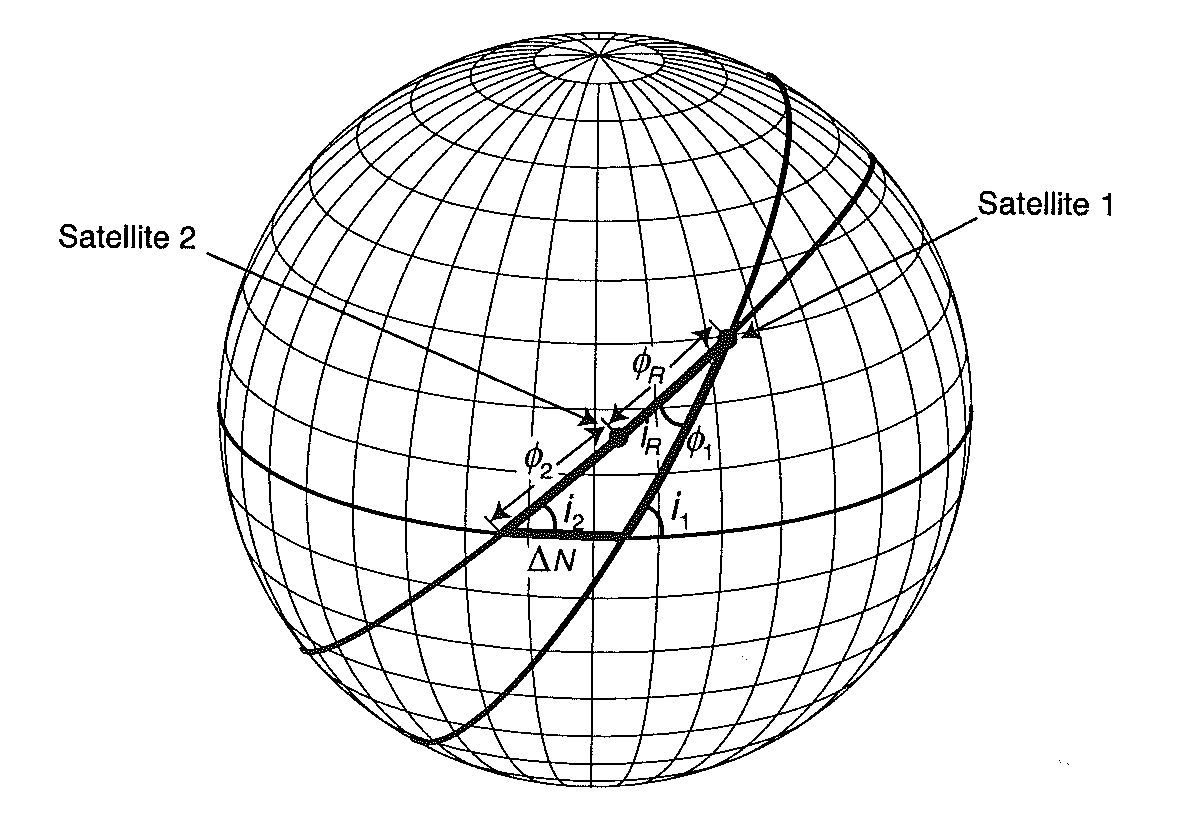
\includegraphics[width=0.8\textwidth, angle=0]{img/relativeMotion.png}
\label{fig:relativeMotion}
\caption{The relative motion of co-altitude satellites in circular orbits. Relative inclination and relative phase are shown. \emph{Source: \cite{constDesign}}}
\end{figure}

Two cases of cross-track motion exist: 

\begin{enumerate}
	\item Inclination of each orbital plane is the same ($i_1 = i_2 = i$) while the ascension nodes have a certain angular separation. This is the most common constellation type.
	\item Inclinations vary with each orbital plane. In this case all satellites can also have the same node of ascension, however this might not necessarily be the case.
\end{enumerate}

Out of the two cases, the most convenient one for the purpose of formation flying is method number 1. Since orbit precession is a function of only the inclination, it is smart to keep it the same for all satellites. This method is demonstrated in figure \ref{fig:intersection} on page \pageref{fig:intersection}.

\begin{figure}[ht!]
\centering
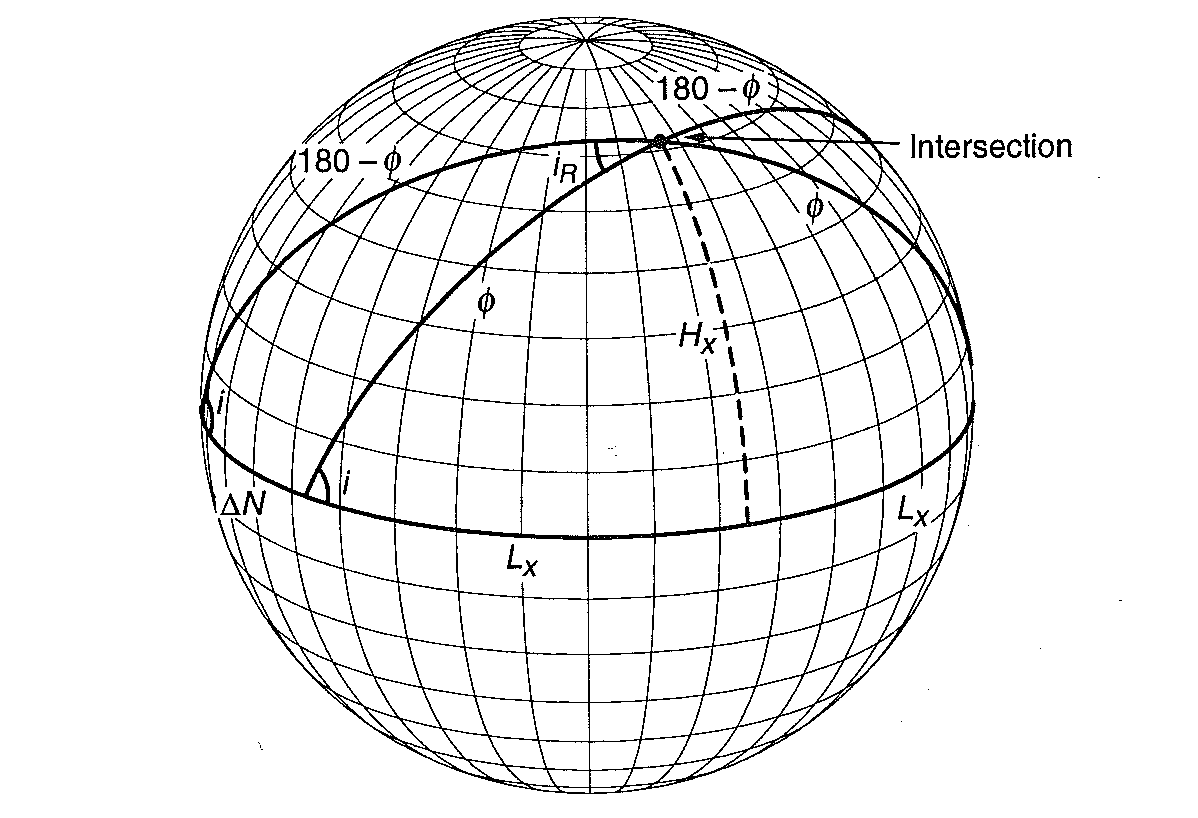
\includegraphics[width=0.8\textwidth, angle=0]{img/intersection.png}
\label{fig:intersection}
\caption{Intersection of two orbits with the same inclination. \emph{Source: \cite{constDesign}}}
\end{figure}

In the above said figure the $\Delta$N is the angular separation between the ascending nodes on the equator. For this case the following equations can be used:

\begin{equation}
cos i_R = cos^2i+sin^2i cos \Delta N
\label{ir}
\end{equation}
\begin{equation}
\phi_R = (T_2-T_1)n+ \Delta \phi
\label{phir}
\end{equation}
where
\begin{equation}
\Delta \phi = 180 - 2 \phi
\label{deltaPhi}
\end{equation}
\begin{equation}
tan \phi = \frac{tan ( 90 - \Delta N / 2)}{cos i}
\label{tanphi}
\end{equation}

Furthermore the relations for minimum and maximum angular separation of the two satellites are given:

\begin{equation}
sin ( \frac{\lambda_{min}}{2} ) = sin ( \frac{ \phi_R }{2} ) cos ( \frac{i_R}{2} )
\label{lambdamin}
\end{equation}

\begin{equation}
cos ( \frac{\lambda_{max}}{2} ) = cos ( \frac{ \phi_R }{2} ) cos ( \frac{i_R}{2} )
\label{lambdamax}
\end{equation}

The angular separation is a very important factor. To be able to determine the BRDF of the surface being observed, the separation should be as large as possible, as the BRDF is an angular property. However, for the purposes of \ac{ADCS} and inter-satellite communications, the separation should be kept small. Figure \ref{fig:earthangle} demonstrates the geometry of separation of the satellites.

\begin{figure}[ht!]
\centering
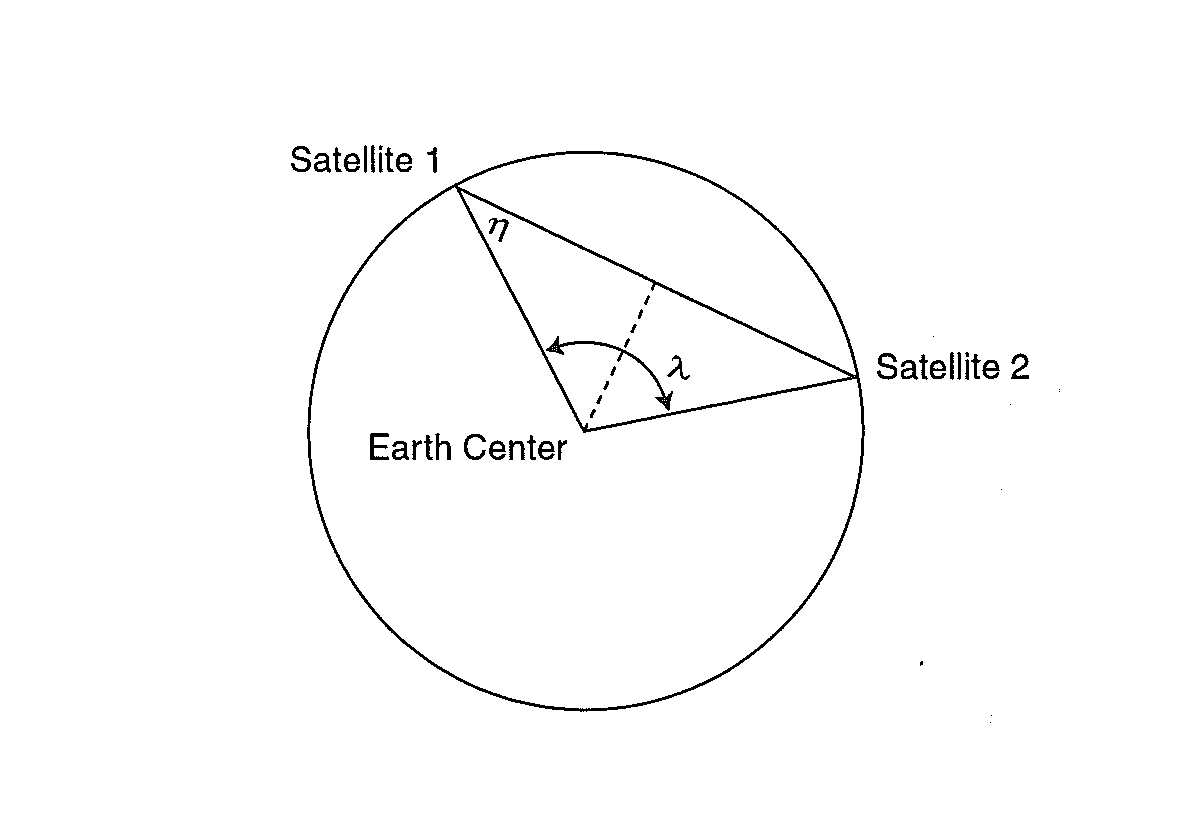
\includegraphics[width=0.8\textwidth, angle=0]{img/geometry.png}
\label{fig:earthangle}
\caption{Geometry of angular seperation. \emph{Source: \cite{constDesign}}}
\end{figure}

All of the above equations are in terms of degrees. Based on these relations it is possible to calculate the relationships between the equatorial angular separation and relative inclination, relative phase and the minimum and maximum angular separation.

\begin{figure}[ht!]
\centering
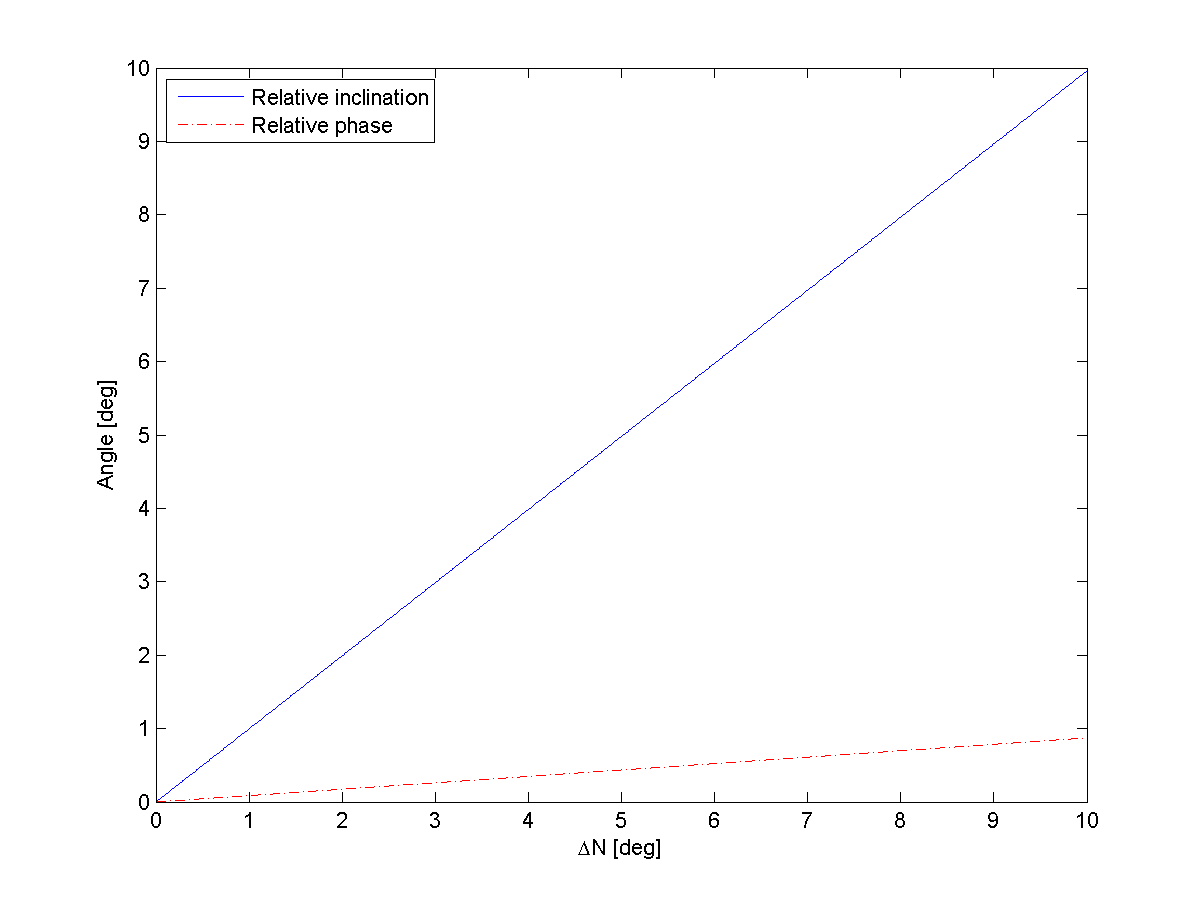
\includegraphics[width=0.8\textwidth, angle=0]{img/relativeInc.png}
\label{fig:relativeI}
\caption{$i_R$ and $\phi_R$ vs. equatorial angular separation. Orbit inclination of $85^o$.}
\end{figure}

\begin{figure}[ht!]
\centering
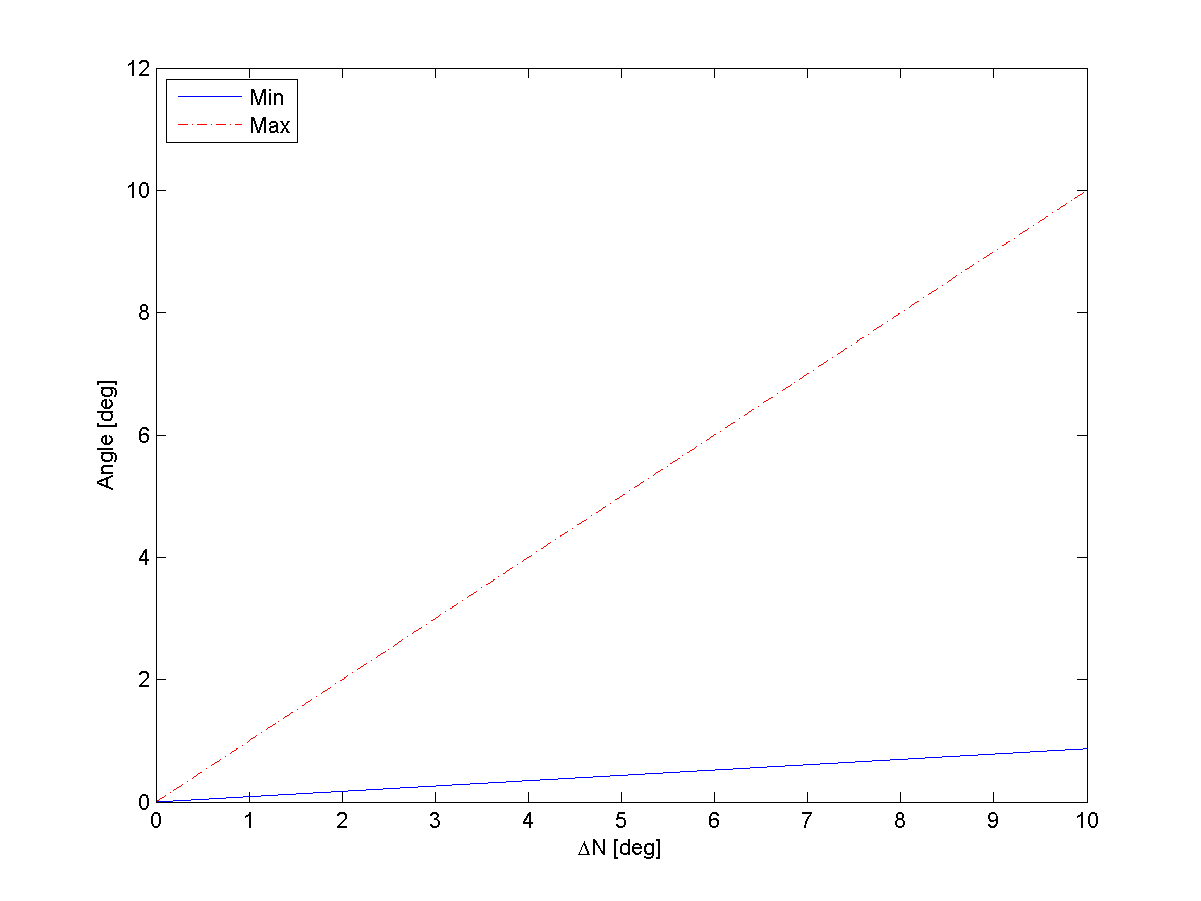
\includegraphics[width=0.8\textwidth, angle=0]{img/angularSeperation.png}
\label{fig:relativeSep}
\caption{Minimum and maximum angular separation vs. equatorial angular separation. Orbit inclination of $85^o$.}
\end{figure}

It is obvious from figures \ref{fig:relativeI} and \ref{fig:relativeSep} that the relative inclination and the maximum angular separation are almost equivalent to the equatorial separation. 

From the point of view of instrument pointing, the receiver should be at such separation from the emitter that the return signal is in the range of 1 to 30 degrees with respect to emitter nadir.
\subsection{Number of Satellites}
\label{mtrSwarmSatNum}
WRITE ABOUT NUMBER OF SATELLITES
\subsection{Stationkeeping}
\label{mtrSwarmStationkeeping}
WRITE ABOUT STATIONKEEPING
\subsection{Collision Avoidance}
\label{mtrSwarmCollision}
WRITE ABOUT COLLISION AVOIDANCE
\subsection{Conclusions and Recommendations}
\label{mtrSwarmRec}
\end{document}